%課題研究レジュメテンプレート ver. 1.0

\documentclass[uplatex]{jsarticle}
\usepackage[top=20mm,bottom=20mm,left=20mm,right=20mm]{geometry}
\usepackage[T1]{fontenc}
\usepackage{txfonts}
\usepackage{wrapfig}
\usepackage[expert,deluxe]{otf}
\usepackage[dvipdfmx,hiresbb]{graphicx}

\makeatletter
  \renewcommand{\section}{%
    \if@slide\clearpage\fi
    \@startsection{section}{1}{\z@}%
    {\Cvs \@plus.5\Cdp \@minus.2\Cdp}% 前アキ
    {.5\Cvs \@plus.3\Cdp}% 後アキ
    %{\normalfont\Large\headfont\raggedright}}
    {\normalfont\raggedright}}

  \renewcommand{\subsection}{\@startsection{subsection}{2}{\z@}%
    {\Cvs \@plus.5\Cdp \@minus.2\Cdp}% 前アキ
    {.5\Cvs \@plus.3\Cdp}% 後アキ
    %{\normalfont\large\headfont}}
    {\normalfont}}

  \renewcommand{\subsubsection}{\@startsection{subsubsection}{3}{\z@}%
    {\Cvs \@plus.5\Cdp \@minus.2\Cdp}%
    {\z@}%
    %{\normalfont\normalsize\headfont}}
    {\normalfont}}
\makeatother
%ここから上を編集する必要はない.





\title{\vspace{-14mm}クラウドファンディングにおいてTwitterが果たす役割の調査}
\author{PMコース 矢吹研究室 1242131 吉野 聡志}
\date{}%日付を入れる必要はない.
\pagestyle{empty}%ページ番号は振らない.
\begin{document}
\maketitle





\section{研究の背景}

資金調達をする手段のひとつとしてクラウドファンディングが存在する.クラウドファンディングとは,ある目的のために不特定多数の人から資金を集める行為,またそのためのWebサービスのことである.大衆 (crowd) と財政的支援 (funding) からなる造語であり,ソーシャルファンディングとも呼ばれる.クラウドファンディングを実施する者は,インターネットを利用して人々に資金提供を呼びかけ,必要とする金額が集まったら目的を遂行する.クラウドファンディングを実施するためのWebサービスサイト上にあるプロジェクトのページを見ると,短期間の募集で多くの人から小口のお金を集めていることが分かる.期間内に目標額に達しなかった場合目的が遂行されることはなく,支援する際に振り込んだお金が勝手に引き落とされることもない.出資への見返りの有無などで「寄付型」「購入型」「投資型」などに分けられる.日本では2011年の春頃にREADYFOR?やCAMPFIRE等のサービスが開始され,東日本大震災関連の復興支援事業で多額の資金調達に成功したことからクラウドファンディングが注目を集めるようになった.

また,世界的に人気なSNSのひとつとしてTwitterが存在する.ユーザが「つぶやき」と呼ばれる140字以内の短い記事を書き込み,他のユーザがそれを読んだり,返信をすることでコミュニケーションが生まれる.他のユーザのつぶやきを追跡することを「フォローする」といい,自分とフォローしたユーザのつぶやきが同一の画面上にリアルタイムで,時系列に沿って表示される.この画面はタイムラインと呼ばれる.フォローをするのに相手の承認は不要で,自分が閲覧していない間もタイムラインが常に流れていくことから,「ゆるいつながり」が生まれるとされている.また,Twitterにはリツイートという機能が実装されている.これは,他のユーザのつぶやきをそのままの形で自分のフォロワー(そのユーザのつぶやきを追跡しているユーザ)のタイムライン上に表示させるものである.なお,リツイートはTwitterを利用しているユーザの間では俗に「拡散」と呼ばれ,自分のフォロワーに宣伝あるいは周知させるという認識が持たれている.

今日のWebサイト上には,特定の商品やニュースなどの情報をそのページの簡単な見出しやリンクとなるURLを載せた上で各SNS上に投稿し,紹介するためのボタンが設置されていることが多い.これにより,ユーザは自分の趣味や気になった話題などをより簡単に発信できるようになる.このような形で情報を発信することは,ボタンを設置したページがより多くの人の目に触れる機会を与える.企業であれば,自社のサイトにボタンを設置することで一種のマーケティングとして活用することもでき,消費者の注目を大きく集めれば少ない労力で多くの利益を得られることが期待される.また,消費者たちにその企業の名前を定着させるのに効果的である.





\section{研究の目的}



本研究では,クラウドファンディングを行うための各ページに設置されたボタンのうち,Twitter上にそのページの情報を発信する「ツイート」ボタンからつぶやきが投稿され,「ゆるいつながり」の中でその投稿がきっかけとなってパトロン(支援者)が増加する可能性があることに着目した.今回の研究ではツイートボタンからの投稿がクラウドファンディングを成功に導く要因となるのかを分析する.






\section{プロジェクトマネジメントとの関連}

プロジェクトの遂行にはメンバやステークホルダー間での情報共有が重要である.今回の研究では,メンバにはパトロンやつぶやきを見た人々,ステークホルダーには支援を呼びかける者とメンバの関係がそれぞれ当てはまる.これはプロジェクトマネジメントの知識エリアにおいてはプロジェクト・コミュニケーション・マネジメントに該当する\cite{PM2013}.本研究ではTwitterを一種の情報共有の手段として扱う.





\section{研究の方法}

本研究ではまず,クラウドファンディングを実施するプロジェクトのページごとにツイートボタンから投稿されたつぶやきを検索し,一覧にしてまとめる.そのためにTogetterというWebサービスを用いる.このようにしてまとめる理由はTwitterの仕様上,つぶやきそのものが消去されるわけではないが,1週間以上前のつぶやきは検索してもヒットしないため,支援を呼びかける期間が1週間を大きく超えるプロジェクトが多い中でつぶやきを探し出すのが困難になるからである.したがって,つぶやきを保存し,いつでもすぐに研究に利用できるようにする目的でTogetterを用いる.今回はアメリカのINDIEGOGOというクラウドファンディングを行うためのサイトで11/21~12/10に実施されたプロジェクト10個を取り上げ,プロジェクトのページごとにツイートボタンからの投稿をまとめる.

次に,各まとめを参照してつぶやきをしたユーザひとりひとりのフォロワーの数を確認し,プロジェクトごとにフォロワー数の合計値を算出,これをつぶやきの影響度という指標(単位は人とする)として扱う.

最後に合計値とプロジェクトの成否をそれぞれ規準変数として扱い,データマイニングを行うためのツールであるRを用いて決定木を作成する.このようにして,つぶやきの影響度によるプロジェクトが成功する確率の変動を調査する.



%\begin{wrapfigure}[行数]{r}{幅}%行数はオプションだが,調整しないとうまくいかない.
\begin{wrapfigure}[12]{r}{10cm}
\vspace*{-\intextsep}
%\includegraphics[width=図の幅,clip]{ファイル名}\label{参照用ラベル}
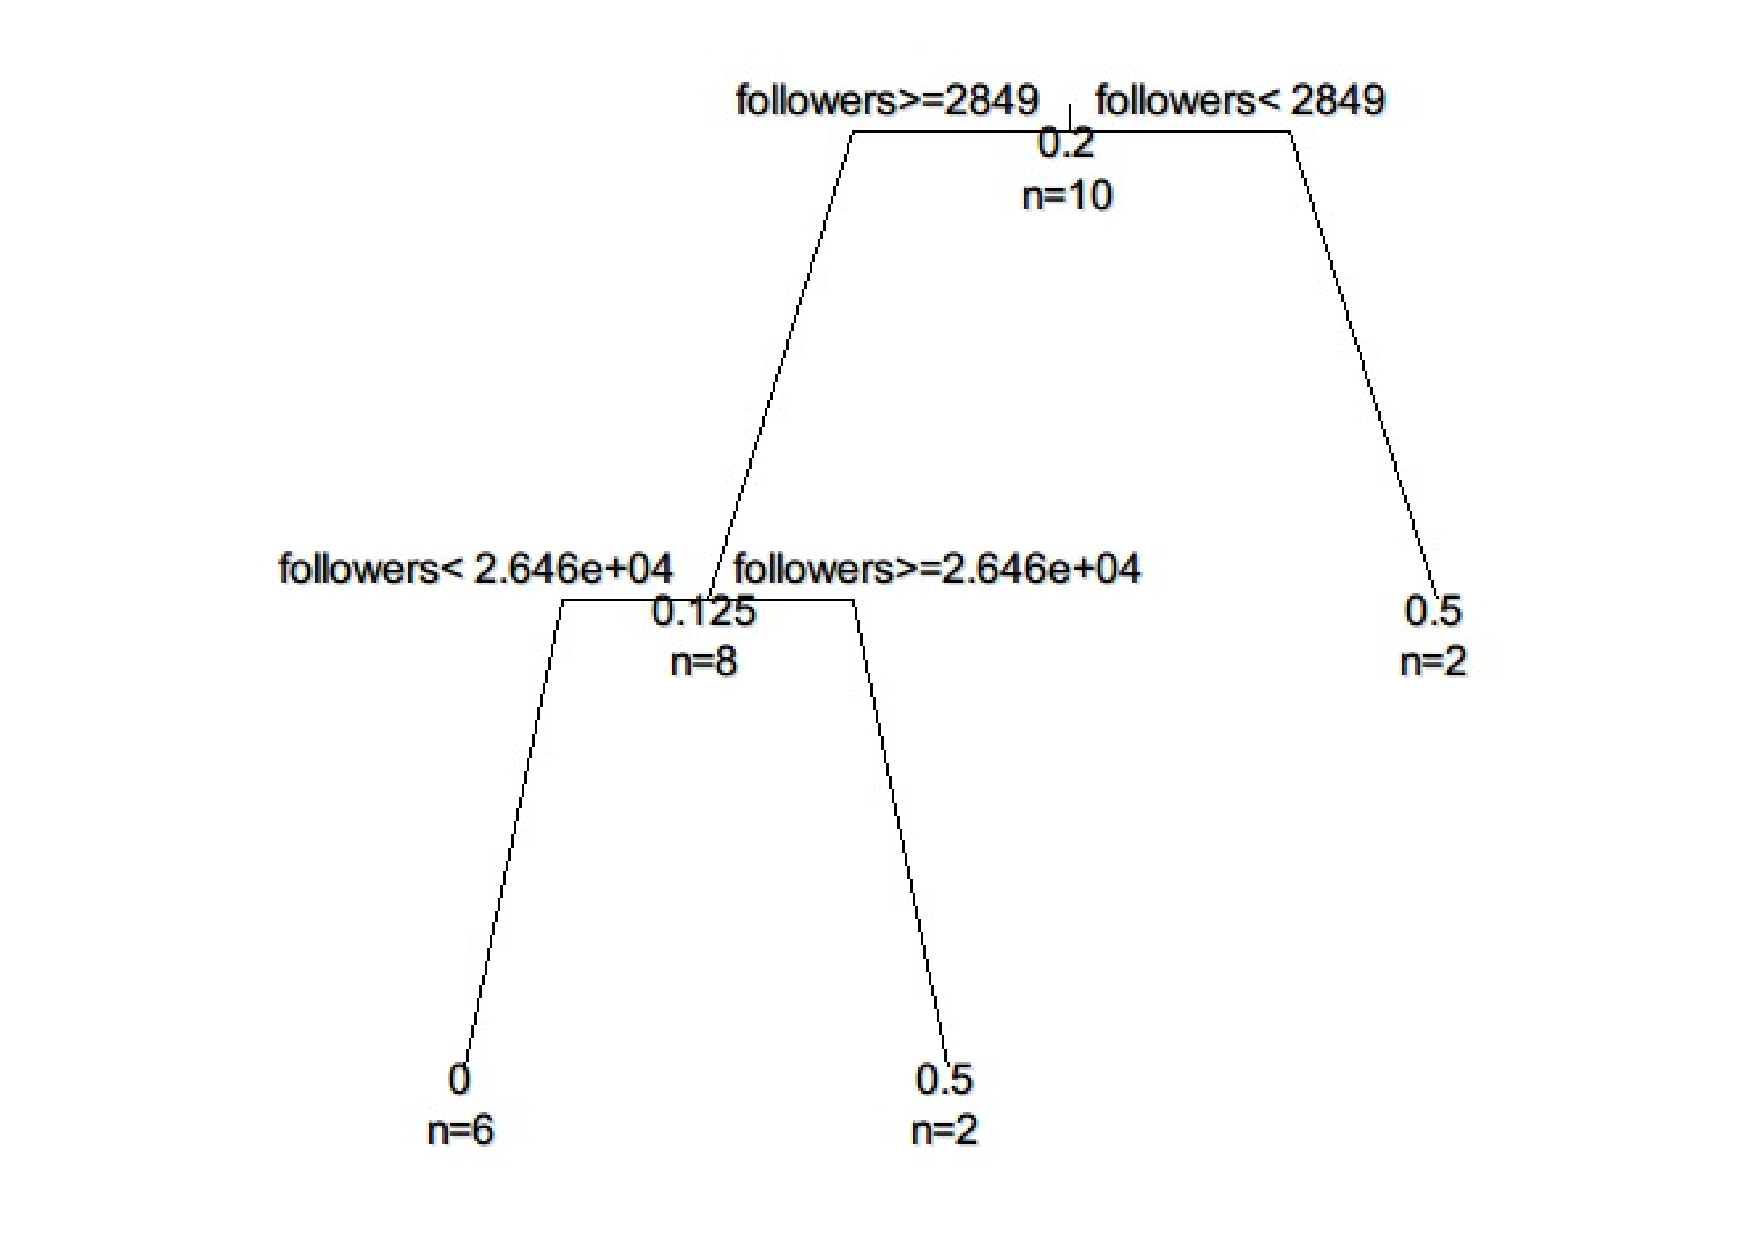
\includegraphics[width=10cm,clip]{images.pdf}
\caption{作成した決定木}\label{サンプル図}
\end{wrapfigure}


\section{現在の進捗状況}

上記の手順で決定木を作成したところ,図1のようになった.つぶやきの影響度が2849人未満の場合プロジェクトは50\%の確率で成功する.しかし,2849人以上だと12.5\%となるという結果が出た.また,後者の結果のうち,つぶやきの影響度が26457.5人以上だと50\%となった.つぶやきの影響度が増加するとプロジェクトの成功率が下がり,2つの変数間には負の相関があるということが分かる.




\section{今後の計画}

今後は以下のように研究を進める.

\begin{enumerate}
\item 調査対象となるプロジェクトの数を増やしたり,他の分析手法も用いて分析を行う.
\item Twitter以外のSNS(FacebookやGoogle+等)の利用状況も含めて調査し,クラウドファンディングとSNSの関係性について考察する.
\item 論文の執筆を行う.
\end{enumerate} 

\bibliographystyle{junsrt}
\bibliography{biblio}%「biblio.bib」というファイルが必要.

\end{document}